%%%%% The Solution (Part 2) %%%%%

\chapter{Implementation: Lesson Plans} \label{ch_teaching}

In order to show how the Processing Abstractions environment introduced in chapter \ref{ch_pa} can be employed for teaching high school students, we have assembled sketches for teaching sequences. Every sequence aims to have students explore further abstractions involved in programming and computer architecture and allows teachers to demonstrate that not just abstractions but also \emph{Sichtenwechsel} are foundational ideas in computer science.

In this chapter, we propose three different sequences. The plans for these sequences list steps from which concrete lessons can be planned.\footnote{\eg according to a model as proposed by Manz and Sch�nenberger \cite{Man20}.} For brevity, we focus on learning steps 2 to 4 in Leisen's teaching model \cite{Lei18}, \ie developing ideas, students working on their own, and discussions of their results.

The main sequence in \ref{sc_lesson_ca} shows how Processing Abstractions is meant to be used for, on the one hand, having students explore the various abstraction levels involved in translating a Processing program to bytecode and running it in the \ac{GT} \ac{VM}, and, on the other hand, discussing computer architecture based on these explorations. This sequence is also meant to better tie computer architecture to preexisting programming knowledge. In particular, if the introduction to programming has already happened in Processing or Python, this allows students to investigate their own programs instead of mainly relying on sample code given by the teacher.

In order for students to best profit from that main sequence, we propose in \ref{sc_lesson_intro} to use Processing Abstractions also for the introduction to programming. This is meant to increase the recall effect in students when returning to programming, and is also meant for students to have programs of their own to investigate in the later sequences. When the limitations of the environment are reached, the move over to the official Processing \ac{IDE} should be seamless: code copied over and run (with the same icon and shortcut) yields the same output and can then be further modified with the full Processing \ac{API} once students are ready.

For diving further into the matter or for students specializing in computer science, we finally propose a third sequence in \ref{sc_lesson_compiler}, which uses the same environment and potentially the same student programs from the first two sequences for teaching the inner workings of a compiler from lexer to optimizer (and potentially again discussing abstractions \emph{per se}).

Finally, in \ref{sc_lesson_other}, we close with a few ideas for how Processing Abstractions could be used as a stepping stone for introducing Smalltalk as a different programming language and \ac{GT} as the moldable environment it is, leading students in specialization courses to molding the provided materials further by \eg extending the Processing \ac{API}, developing new views or starting to work on a language of their own. This can be used to discuss abstractions involved in teaching by revealing the innards of Processing Abstractions.

For all proposed sequences, Processing Abstractions can either be used just for its Processing compiler, runtime environment, and the various views provided. We suggest also considering embedding the full course materials in interactive notebook pages for students to work in at their own pace. Processing Abstractions includes a foundation of such materials in German, which have already been tested with students and adjusted afterwards (see chapter \ref{ch_practice}). When used like this, \ac{GT} can also serve as a digital notebook to students, where they solve tasks directly in the page, add their own notes, and keep their modified examples.

While Processing Abstractions is mainly targeted at high school students, the sequences proposed here could also be used in middle school. For middle schoolers, the exposed user interface would, however, have to be reduced as far as possible to keep it manageable. It could nonetheless work at least in a smaller group with interested and motivated students wanting to step beyond block-based programming languages. For university students, in contrast, there's currently not enough depth available.



\section{Introduction to Programming} \label{sc_lesson_intro}

While the Processing Abstractions environment has been developed for linking programming and computer architecture, it can also be used for an introduction to programming. This should help better link programming and computer architecture for students, since they can start at the same point and reuse the experience already gained and programs already written.


\subsection{Educational objective}

After the introduction, students should be able to \dots
\begin{itemize}
\item work within \ac{GT}.
\item read, write, and understand programs with a limited command set, including working with the implicit animation loop.
\item learn from their mistakes, correct themselves, and not be afraid of breaking things.
\end{itemize}

In the end, students should have a solid foundation for taking on the task of writing a basic but still interesting app or game.\footnote{Possible ideas, which all have been implemented by students, include: Flappy Bird, Geometry Dash, Pong, Doodle Jump, Snake, a quiz, a labyrinth, \etc For most of these, Processing Abstractions provides sufficient support, the main deficit being the lack of keyboard input.}


\subsection{Prerequisites}

Students need experience in using their own computer, including \dots
\begin{itemize}
\item downloading and extracting archives, and
\item dealing with their virus scanner.\footnote{At least under Windows, many scanners flag \ac{GT} as untrustworthy due to its executable lacking a valid signature. Some virus scanners even block the entire download if the archive is distributed over a network.}
\end{itemize}

Additionally, the teacher must prepare their content in \ac{GT} \eg as described in \ref{app_setup} and distribute it. Ensure that the first lesson page will be displayed on the first startup.


\subsection{Introduction to Glamorous Toolkit} \label{ssc_lesson_gt}

Since \ac{GT} will be a new environment altogether for all students, some basics on its usage have to be introduced first within ten minutes:

\begin{instructions}
\item Ask students to download and extract your \ac{GT} distribution as homework for the first lesson. Under Windows, they might run into a first issue with their virus scanner blocking the download, so remind them about what to do in that case.\footnote{With most virus scanners, the warning can be overruled by the user; otherwise they might have to \emph{temporarily} disable the scanner for this one download.}
\item Tell students to start \ac{GT} and open the notebook page about working with \ac{GT} (``Arbeiten mit Glamorous Toolkit'' in the included teaching materials). Also ask them to help their neighbours if they see them struggling. Use the time while students are reading and doing the first tasks to ensure that everyone has managed to get \ac{GT} running.
\item Introduce \ac{GT} as an interactive notebook similar to what students already know from class.\footnote{Many schools have standardized their IT infrastructure and use the Microsoft 365 Office Suite, which includes OneNote.} One main difference will be that additional views will open to the side, hiding the table of contents. So show them how to get back by selecting the left-most view (through the blue dots at the center top) and expanding it (through the \faPlusCircle\ at the top left).
\item If you want students to be able to take notes of their own inside \ac{GT} notebooks, show them how to move a page to their local knowledge base (where it can be backed up individually) and how to create and structure new paragraphs (\ct{Ctrl+Enter}, \ct{Alt+Shift+Arrow}). Markdown syntax for formatting does not have to be introduced explicitly, as that can be replicated by students by inspecting your content.
\item Finally, keep in mind \ac{GT}'s ability to be inspected at every level and point more advanced students towards using these (\eg by \ct{Ctrl+Shift+Alt+Click} anywhere, by double-clicking on list items, or by going through the different views of an object).
\end{instructions}

Please note that as described in \ref{sc_gt}, \ac{GT} is bleeding edge technology and might not always behave the way you and your students have become used to: Since notebook pages are rendered progressively, scrolling won't always work smoothly (and will scroll inner content, if the mouse cursor isn't positioned at a page's border); occasionally unexpected error messages cause a debugger window to pop up, which has to be closed again; and sometimes the keyboard modifiers may get stuck, resulting in shortcuts no longer working (which is resolved by switching to a different app and back).


\subsection{Lesson Plan}

Since this isn't the focus of this thesis, we won't go into much detail about introducing programming, but just summarize what might work within the provided environment:

Start top down as suggested in \ref{ssc_top_down} from either abstract art or games\footnote{Most one-tap games should work; \eg \url{https://www.lessmilk.com/almost-pong/} has reasonably simple gameplay with minimalist visuals.} and start dissecting how this concrete entity might be described, first in natural language and then in formalized language.

Then follow Reas and Fry \cite{Rea14} and introduce the Processing language (see \ref{sc_processing}), by starting with a sequence of statements with few commands (\eg \ct{size}, \ct{rect}, \ct{ellipse}, and \ct{fill}), and then sequentially introducing comments, colors, variables, and arithmetic, the animation loop, conditions, and interactivity.

Every concept can be described on a notebook page with given examples for first exploring the effects of a command and its arguments\footnote{Students may either describe the expected behavior and then verify that their expectation matches the outcome, or, as a less taxing alternative, try given or random values and then describe their observations. Variations consist \eg in a student describing desired behavior and then (another student) trying to achieve this.} and then later using the concept for solving problems by starting from a skeleton program (see figure \ref{fig_screenshot_introduction} for an example of both).

\begin{cfigure}[fig_screenshot_introduction]{Excerpt from an interactive notebook page with exploratory and live programming tasks.}
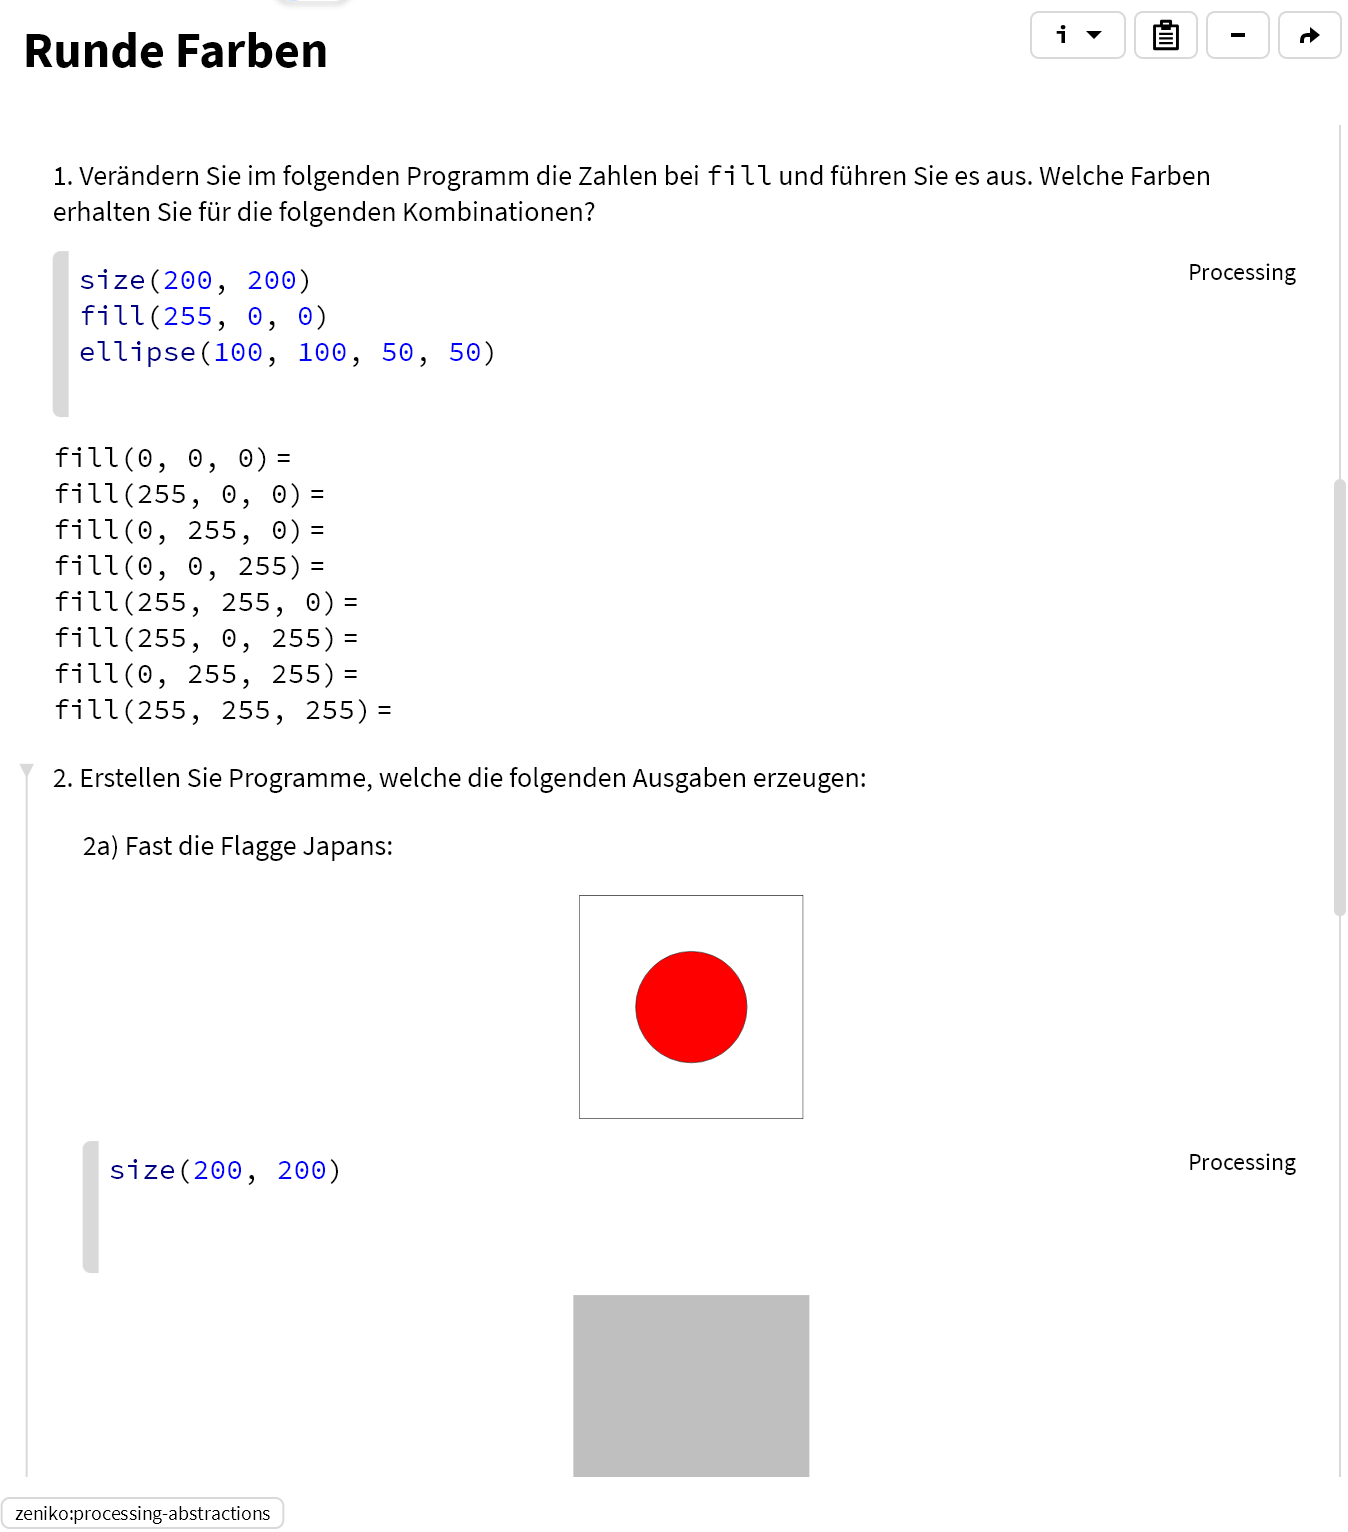
\includegraphics[width=.7\textwidth]{screenshot_introduction}
\end{cfigure}

At the beginning, debugging will only consist in modifying values and observing live changes until the desired output is reached. At later stages, the step-by-step execution views will be useful, where executed expression, variable values, and visual output are displayed side by side and execution can be played forward and also in reverse.

Quicker and more proficient students could also already, at this point, start to delve deeper: The third and fourth execution icons will lead them to discover by themselves what lies under the hood.

Sample content for this is included in the \emph{Unterrichtsmaterialien} of Processing Abstractions as ``\emph{Programmieren mit Processing}''.



\section{Lesson on Computer Architecture} \label{sc_lesson_ca}

The main objective of this thesis was to demonstrate how understanding of what happens when executing a program could be improved by having students perform a \emph{Sichtenwechsel}. The same goes for the other way around, where computer architecture is explained in more concrete form by tying it to previous programming experience.

Introductions to computer science, which extend beyond a pure programming course, often contain lessons on computer architecture. \eg the curriculum \cite[p.\,145]{Erz16} asks for students to ``know how computers and networks are structured and work''.

We again propose to approach this task top down (see \ref{ssc_top_down}) and move along the path specified in figure \ref{fig_multitier}. This will be outlined here, with validation of part of this approach following in \ref{sc_validation_ca}.

With respect to manageability (see \ref{ssc_manageability}), it is proposed to mostly skip the inner workings of a compiler and treat that in a separate sequence (maybe only for students specializing in computer science).


\subsection{Educational objective}

After these lessons, students should be able to \dots
\begin{itemize}
\item explain the concepts of (virtual) machine, memory, stack, machine language, and program counter (with reference to a von Neumann model).
\item elaborate why machine language must be different from a high-level language such as Processing.
\item explain why some commands are slower than others.
\item connect their knowledge about encodings with how values and machine code are stored.
\item consequently understand how one of their programs might be run on actual hardware and document their understanding with correct terms.
\end{itemize}


\subsection{Prerequisites}

Students must already have basic programming skills in a high-level language. In particular, they must know about variables and loops. If they don't know Processing or at least Python yet, a brief introduction (maybe along the ideas proposed in \ref{sc_lesson_intro} above) is required.


\subsection{Lesson Plan}

Whereas Nisan and Schocken \cite{Nis21} introduce their bottom up course with a top-down overview, we propose doing the same in reverse for this top-down approach:

\begin{instructions}
\item Start with a brief repetition on programming by giving students a few quickly solved tasks (including one about the animation loop, where at least the skeleton structure is given). If this is the students' first encounter with \ac{GT}, use this opportunity to introduce it (see \ref{ssc_lesson_gt}).
\item Show students the innards of a computer and ask where their programs reside in there. Use this for discussing hard drives and volatile memory, and a repetition about encodings and how everything boils down to \ct{1}s and \ct{0}s (or current and no current, respectively).
\item Briefly start at the desired lowest abstraction layer, \eg (light) switches, and explain how they are used for creating processors.
\item Ask students about games they play, and have them describe possible player \emph{actions} and compare them with actual player \emph{input}.\footnote{Alternatively, if starting from art instead of games, decompose drawing \eg a house into individual brush strokes.} This repeats top-down abstraction decomposition, as maybe already encountered in the introduction to programming lessons, and allows teachers to bring the foundational idea of multitier architectures back to students' minds.\footnote{Multitier architectures might already have been discussed as part of networking lessons.}
\item Have students go back to a sample or one of their own Processing programs, and let it (again) be displayed in machine code. Provide them with several examples, \eg with variable assignment, with conditionals and loops, and let them assemble the required machine code mnemonics and byte values.\footnote{Ideally, distribute the examples over small student groups, two groups per example.} Suggest variations for the example, so that even with less programming experience, they may find regularities.
\item Collect their findings and group their arguments: pushing to the stack/accumulator (machine codes 0--83), returning (88--94), binary arithmetic and comparison operations (96--111), common commands (112--127), message sending/function calls (128--175), jumps (176--199), storing results (200--216), combined multi-byte instructions (first byte: 224--255) \cite[p.\,12]{Ber14}.\footnote{Students should, at this point, be able to explain where these seemingly odd number ranges stem from.}
\item Take a step back: What is relevant for running a program? This should yield memory, (arithmetic) operations, input and output, and control flow. Let students go back to their examples and see if Processing code for one or multiple of these core concepts maps to the found machine codes.
\item Introduce von Neumann architecture (see figure \ref{fig_von_neumann}) as an abstraction of the encountered concepts. What physical parts of a computer belong to the idealized concepts?
\item Discuss \acp{VM} in comparison to physical machines\footnote{\acp{VM} being used for portability reasons, such as the Smalltalk \ac{VM}, the Java \ac{VM}, Microsoft's dotNet \ac{VM} or any browser's \ac{VM} for WASM.} and the difference of stack and register machines, \acp{VM} tending to the former and physical machines to the latter.
\item Go back to Processing and inspect a combined execution view (see figure \ref{fig_screenshot_vm_execution}). By stepping forward and backward, students should be able to observe the role of the stack and the program counter. Let them explore execution flow and write down what role the program counter has and what the calling convention for Processing \ac{API} calls seems to be.
\item As a break or maybe as homework, let students play Human Resource Machine\footnote{The Hour of Code edition is free to download for Windows and macOS.} \cite{Tom15}, which introduces students to a different architecture. The first six levels should be doable for everybody, with quicker students finding sufficient challenges later on.\footnote{You can also come back to this during compiler lessons, as Human Resource Machine has players implement various optimizations as additional challenges.}
\item Compare the two instruction architectures with regard to expressivity and register- \emph{vs.} stack-based design.

\item Finally, treat circuits, logic gates, transistors, and maybe down to silicon outside of \ac{GT} to the desired depth.
\end{instructions}

\begin{cfigure}[fig_von_neumann]{Von Neumann architecture.}
\begin{tikzpicture}

\node [draw, rectangle, text width=1.5cm, align=center, minimum width=2cm, minimum height=2cm] (input) at (-5, 0) {Input Device};
\node [draw, rectangle, text width=1.5cm, align=center, minimum width=2cm, minimum height=2cm] (output) at (5, 0) {Output Device};
\node [draw, rectangle, minimum width=5cm, minimum height=7cm] (machine) at (0, 0) {};

\node [draw, rectangle, minimum width=4cm, minimum height=4cm] (cpu) at (0, 1) {};
\node [draw, rectangle, minimum width=4cm, minimum height=1cm] (memory) at (0, -2.5) {Memory Unit};

\node at (0, 2.5) {Central Processing Unit};
\node [draw, rectangle, minimum width=3.5cm, minimum height=1cm] at (0, 1.5) {Control Unit};
\node [draw, rectangle, minimum width=3.5cm, minimum height=1cm] at (0, 0) {Arithmetic Logic Unit};

\draw [-{Latex[length=5mm]}] (input) -- (machine);
\draw [-{Latex[length=5mm]}] (machine) -- (output);
\draw [->, transform canvas={shift={(-5pt, 0)}}] (cpu) -- (memory);
\draw [<-, transform canvas={shift={(+5pt, 0)}}] (cpu) -- (memory);

\end{tikzpicture}

\end{cfigure}



\section{Lesson on Compilers} \label{sc_lesson_compiler}

Once students have an approximate understanding of what a program must be transformed into in order to be run on actual hardware or inside a \ac{VM}, the question remains as to how the transformation from source code to machine code happens.

While this is not usually the focus of a general introduction to computer science beyond the superficial treatment occurring during the lessons on computer architecture, this is quite relevant for students specializing in computer science.

However, using the environment presented here, this topic could just as well be used either for all students or for quicker students to work on mostly by themselves. Part of the lesson presented here has indeed been validated under these circumstances (cf. \ref{sc_validation_compiler}).


\subsection{Educational objective}

After these lessons, students should be able to \dots
\begin{itemize}
\item explain the difference between high- and low-level languages.
\item enumerate the steps required during compilation, using proper terminology (lexer, parser, transpiler, compiler, optimizer).
\item connect this knowledge with their knowledge of computer architecture and programming.
\end{itemize}


\subsection{Prerequisites}

Students must have experience in programming and computer architecture, \eg from the lessons described above (cf. \ref{sc_lesson_intro} and \ref{sc_lesson_ca}). It helps if their programming experience is based on Processing or at least Python. Additionally, they need to have \ac{GT} installed and introduced (see \ref{ssc_lesson_gt}).


\subsection{Lesson Plan}

The natural way to progress on understanding a compiler is top down, which is the same as the chronological order:

\begin{instructions}
\item Before starting to fill in the content missing from the previous lesson on computer architecture, begin with a repetition on how a program is run in a \ac{VM} (see figure \ref{fig_screenshot_vm_execution}), letting students run again a given program or one of their own, and seeing into what commands their code was translated.
\item As an analogy, analyze with students how they would go about translating an unknown language using just a dictionary: splitting the text into words where punctuation yields some structure; then looking words up (where again several words might belong together for the sake of translation\footnote{Compare \eg the meanings of ``to see'', ``to see to'', ``to see through'' and ``to see out''.}); writing the translation down; and finally rewriting it, so that it sounds more akin to how you would write it in the target language. This analogy yields a fitting overview of the different steps involved.
\item Let students work through discovering the individual concepts encountered:
\begin{itemize}
\item Have them compare a program and the resulting lexed tokens: What modifications to a program result in different tokens, what modifications don't cause changes? What does this correspond to in the analogy about translating a natural language?
\item Have them compare the abstract syntax trees resulting from their program(s). Are they able to explain how the parser structures the tokens together? How would they proceed if all they saw were just two tokens? (For this, use a view of tokens showing just two lines.)
\item Discuss how a recursive descent parser works through tokens. Since Python and thus Processing based on Python uses indentation for command grouping, also highlight the need for tracking indentation at least per statement.
\item Optionally have students compare given Processing source code with the resulting \ac{AST} and transpiled Smalltalk: How literal is the translation? What is different between Processing and Smalltalk? Have them try to invent a syntax of their own that is easier to map to the \ac{AST} (and later discuss Lisp and Forth syntaxes as examples for alternative, easier to parse syntaxes\footnote{Views for variants of both are available.}).
\item Since usually an \ac{IR} is directly produced from an \ac{AST}, collect common statement types (variable assignment, function calls, loops, \dots), and have them translated live to \ac{IR}. Let students work out common patterns to see what translation might take place.
\item Have views for \ac{IR} and actual Smalltalk bytecode side by side for students to figure out what transformations remain and why these might be required (comparing with their knowledge from computer architecture lessons).
\item Should students have prior experience with Human Resource Machine \cite{Tom15}, have them translate Processing to a program in that game's simplified language and translate code for a level of that game back to Processing (and from that Smalltalk bytecode with the environment's help).
\item For the final step, offer some simple code examples that can obviously be simplified.\footnote{\eg \ct{print(1+1+1+1+1)} or \ct{for i in range(10): pass}, both of which should be trivially optimizable}. What optimizations are present in the \ac{IR} and which in bytecode? What patterns could be optimized? Also discuss the difference of optimizing for size, for speed, and for quick compilation.\footnote{For players of Human Resource Machine, the first two are the bonus challenges in all later levels.}
\end{itemize}
\item What can't be shown yet using Processing Abstractions are the equivalent of optimizations within a processor (or already the x86, IA64, \etc code produced by the Just in Time compiler). However, students should, at this point, have sufficient understanding of the various transformations that they might be able to understand what happened \eg with the Spectre attack \cite{Koc19} and why understanding of machine code might be relevant for timing attacks.
\end{instructions}



\section{Further Lesson Ideas} \label{sc_lesson_other}

Whereas the environment presented here is mainly targeted at introductory high school classes, it might also be employed in a specialization course. Since this isn't this thesis' focus, we will just list a few ideas:

\begin{itemize}
\item Smalltalk is a rather elegant language and has aged quite well. It can still be used to introduce students to pure object-oriented programming with a somewhat unusual syntax for them, and such an introduction could use transpilations from Processing Abstractions as a stepping stone, if students have already used it.
\item Since the code provided here is run dynamically in \ac{GT}, it can also be molded further, \eg to implement as of yet missing support for object-oriented programming.
\item The provided code might also be used as a template for students to implement their own programming language or see if they manage to write an interpreter for one of the two provided prefix and postfix pseudolanguages.\footnote{This might already have been discussed in the compiler lessons above. Very briefly, a program such as \ct{a = 42; print(a)} is translated to \ct{(= a 42) (print a)} and \ct{\$a 42 = a print}, respectively, which both should be simple enough to parse.}
\item Finally, Processing Abstractions allows one to drive the point home that abstractions leak by showing that teaching environments, \acp{IDE}, or, in fact, any app can be dissected, thereby revealing lower architectural layers, and modified at these lower layers.
\end{itemize}
